\chapter{Projeto do datalogger}
\label{chap:metodologia}

% \section{Motivação}

% A escolha entre uma dessas soluções, deve levar em conta o tipo de aplicação e o nível de criticidade dos dados levantados. Para levantamento de dados de temperatura de salas de armazenamento de vacinas, ou da umidade relativa do ar em uma cultura agrícola e afins, a escolha de um \textit{Datalogger} se mostra ideal. 

\section{Escopo de projeto}


% Definir o escopo do projeto foi o ponto de partida do desenvolvimento do dispositivo datalogger. Para isso, foi então definido que deveria ser desenvolvido um datalogger que fosse capaz de ler, persistir e disponibilizar os dados coletados à partir da leitura da temperatura, umidade relativa e luminosidade do ambiente em que ele esteja instalado. 

% A persistência dos dados coletados deve idealmente ser feita em uma mídia que removível que pudesse manter os dados armazenados por um longo período de tempo e que também seja capaz de suportar temperaturas um maiores que a temperatura ambiente. Além disso, os dados devem ser escritos de forma que seja facilitada a importação deles para ferramentas de visualização de dados. 

A ideia principal do projeto é desenvolver um datalogger cujo custo de aquisição não seja muito alto, dado suas características técnicas. Com isso em mente, foi definido que o datalogger deveria ser um dispositivo capaz de ler temperatura, umidade relativa e luminosidade do ambiente em que ele estiver instalado. 

Essas leituras devem ser realizadas periodicamente de forma que o intervalo entre cada leitura esteja na casa dos segundos, se possível, e devem ser armazenadas em uma mídia de armazenamento de massa removível. Essa mídia deve manter os dados guardados por um período de tempo  de pelo menos um ano e suportar variações de temperaturas ligeiramente maiores ou menores que a temperatura média do local de instalação.


%  Complementar aqui o escopo

\section{Levantamento das especificações técnicas do hardware}

Realizando a análise do escopo definido, foram então levantadas as especificações que o hardware proposto deve atender. À partir dessas especificações será então criado uma arquitetura para o hardware, que elencará quais componentes, protocolos e afins deverão ser adotados.

    \begin{enumerate}
        \item Possuir a capacidade de ler a temperatura do ambiente;
        \item Possuir a capacidade de ler a umidade relativa do ambiente;
        \item Possuir a capacidade de ler o nível de luminosidade do ambiente;
        \item Possuir alternativa de alimentação direta ou via bateria;
        \item Leitura de sensores via interfaces I2C, SPI e/ou UART;
        \item Formatação dos dados lidos dos sensores para auxiliar no envio e/ou coleta;
        \item Persistir os dados em um cartão SD para a coleta manual dos dados;
        \item Persistência dos dados coletados por no mínimo 45 dias;
        % \item Interface de comunicação via rádio LoRa;
        % \item Envio periódico dos dados guardados via LoRaWan;
        \item Possuir interface de interação com o usuário;
        \item Permitir a configuração da taxa de amostragem das variáveis lidas;
        % \item Permitir o envio de dados coletados via interface de comunicação sem fio;
        % \item Permitir o recebimento e aplicação de configurações via interface de comunicação sem fio;
        % \item (Ideia pra placa: Deixar uma interface pra gravação do firwmare)
        % \item Possuir proteção contra intempéries;
        % \item Preferencialmente escolher componentes com propriedades de operação da classe automotiva; 
        % \item Alertas para quando algum dado lido extrapolar um valor pré-configurado;
        % \item Possuir um display lcd ou oled pra ajudar na interação com o usuário;
        % \item Ser possível expandir a quantidade de sensores facilmente e de forma plug\&play;
        % \item Possuir possibilidade de atualização de firwmare over-the-air;
        % \item Possuir células fotovoltaicas para recarregas a bateria;
        % \item Possuir circuito de recarregamento das baterias;

    \end{enumerate}

\section{Definição da arquitetura de hardware}

Tendo sido levantados as especificações do projeto, esses são analisados a fim de se criar uma arquitetura de hardware do projeto. Fazem parte dessa arquitetura o diagrama de blocos do hardware proposto, que irá nortear a definição de que quais componentes que serão necessários para a construção do dispositivo. 

Junto ao levantamento dos componentes, também são elencado quais propriedades eles deverão possuir para que as especificações do projeto sejam atendidos. Uma vez que isso seja feito, é então dado início a seleção desses componentes no mercado de componentes eletrônicos de acordo com o especificado na etapa anterior de levantamento de componentes.

\subsection{Diagrama de blocos}

No diagrama de blocos do dispositivo datalogger proposto, cada bloco é um objeto que representa um componente que deve fazer parte da do hardware. Além disso, são também elencados as interfaces de comunicação, se necessário, que cada objeto deverá ter com outros objetos. 

Analisando as especificações técnicas são definidos quais objetos deverão compor  o hardware. Alguns desses objetos podem ser compostos de objetos menores, dependendo do nível de complexidade que eles apresentam. Assim, o seguintes objetos são definidos:

 \begin{itemize}
     \item Unidade de processamento;
     \item Sensor de luminosidade;
     \item Sensor de temperatura; 
     \item Sensor de umidade;
     \item Unidade de alimentação;
     \item Unidade de interface de usuário;
    %  \item Unidade de interface de comunicação USB;
     \item Unidade de leitura e escrita de dados em cartão SD;
 \end{itemize}

À partir da definição dos objetos, é então elaborado o diagrama de blocos do dispositivo a ser desenvolvido. O diagrama deste projeto segue abaixo.

    \begin{figure}[h!]
            \captionsetup{width=16cm}
    		\Caption{\label{fig:datalogger_blocks} Diagrama de Blocos do datalogger}
    		%\centering
    		\UFCfig{}{
    			\fbox{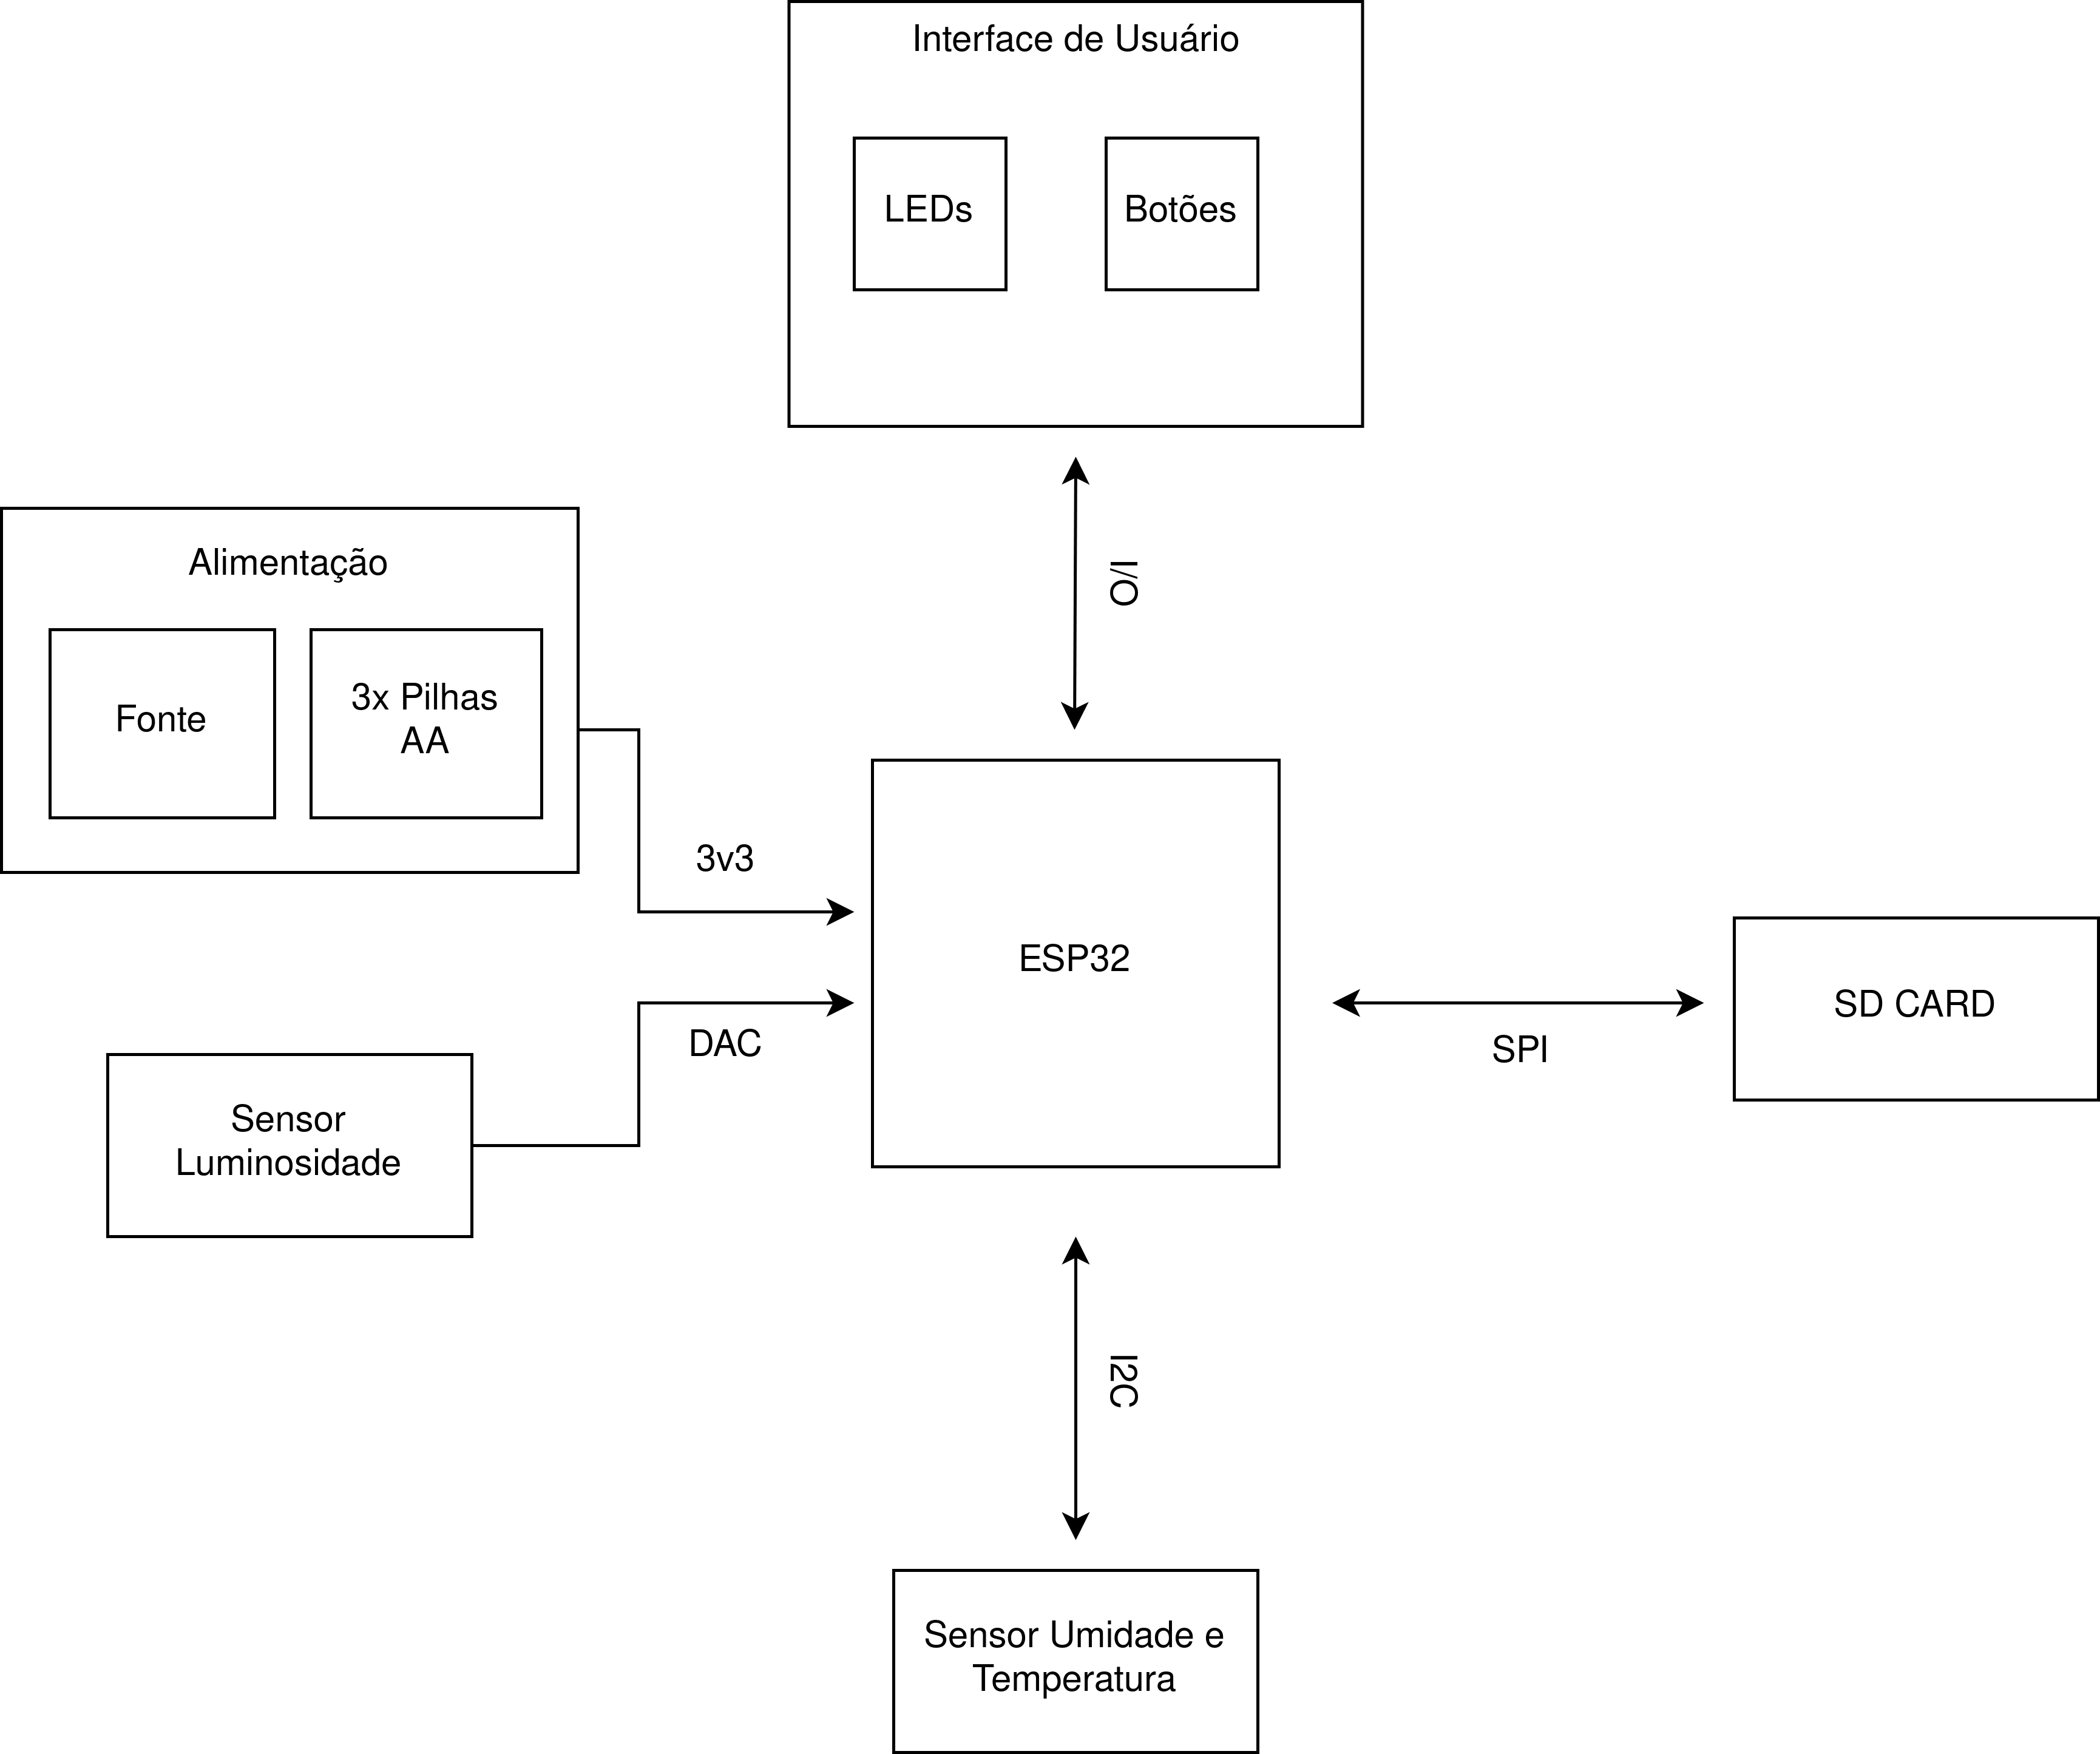
\includegraphics[width=\textwidth]{figuras/capitulo3/datalogger_tcc.drawio.png}}
    		}{
    			\Fonte{elaborado pelo autor (2022).}
    		}	
   \end{figure}

\subsection{Levantamento de tipos de componentes}\label{subsec:levantamento_tipos}


Uma vez que se tenha o diagrama de blocos criado, é dado início ao processo de seleção de componentes. Nesta etapa são analisados as especificações técnicas e o diagrama de blocos do projeto a fim de se levantar quais componentes e quais propriedades esses componentes devem possuir para serem considerados ideais para o desenvolvimento do hardware. 

Assim, para cada objeto do diagrama foram levantado quais tipos de componentes fazem parte da definição desse objeto, com o objetivo de orientar a procura e escolha dos componentes eletrônicos nos distribuidores. Os tipos de componentes levantados seguem abaixo: 

\begin{itemize}
 
 \item Unidade de processamento
     \begin{itemize}
         \item Microcontrolador que opere em 3V3 e possua interfaces de comunicação USART, SPI e I2c;
     \end{itemize}

 \item Sensores de umidade, temperatura e luminosidade; 
  \begin{itemize}
     \item Sensor de umidade relativa e temperatura que opere em 3V3;
     \item Sensor de luminosidade que opere em 3V3;
 \end{itemize}
 
 \item Unidade de alimentação:
     \begin{itemize}
         \item Suporte para baterias do tipo AA;
         \item Circuito que forneça 3,3 V de tensão de alimentação ao hardware;
    \end{itemize} 

\item Unidade de interface de usuário: 

    \begin{itemize}
        \item LEDs multicoloridos;
        \item Botões tácteis.
    \end{itemize}
%  \item Unidade de interface de comunicação USB;
%     \begin{itemize}
%         \item Conector de comunicação USB.
%     \end{itemize}
 
 \item Unidade de leitura e escrita de dados em cartão SD;
     \begin{itemize}
         \item Suporte de leitura de cartão microSD;
     \end{itemize}
 %Acho que aqui é melhor fazer uma análise dos requisitos e ir comentando qual componente atende aos requisitos X e Y.
\end{itemize}

\subsection{Recomendações para seleção de componentes}\label{subsec:recomendacoes_componentes}

Tendo sido levantado quais os tipos de componentes devem fazer parte da construção do hardware proposto, é preciso dar início ao processo escolha dos componentes no mercado de componentes eletrônicos. Contudo, algumas recomendações devem ser feitas antes que essa fase do projeto seja iniciada a fim de se evitar custos adicionais seja durante a fase de desenvolvimento, seja na fase de produção do hardware desenvolvido. 

Assim, como primeira recomendação pode ser destacado a escolha de componentes ativos como microcontroladores,  circuitos integrados de aplicação específica (do inglês Application Specific Integrated Circuit - ASIC) ou semelhantes, que estejam com produção ativa e que tenham um tempo de vida útil garantida pela fabricante de pelo menos 10 anos à partir da data em que projeto inicia sua fase de produção. Essa recomendação visa garantir a longevidade do dispositivo desenvolvido, visto que quando há a descontinuidade de produção ou falta desse tipo de componente no mercado, isso gera um custo extra ao fabricante que se desejar manter seu hardware sendo produzido vai ou precisar adquirir e manter um estoque próprio desses componentes, ou arcar com os custos extras de retrabalho do seu hardware para substituir o componente que está em falta por um equivalente. 

Já para componentes passivos, como resistores, capacitores e afins, é preciso um cuidado semelhante uma vez que também há problema de descontinuidade da produção para esse tipo de componente pelos seus fabricantes. Contudo o processo de substituição por um componente equivalente é mais simples uma vez que um componente com as mesmas propriedades do escolhido inicialmente podem ser produzidos por mais de um fabricante. 

Dessa forma, visando aproveitar essa característica dos componentes passivos é recomendado que no momento da seleção desses componentes sejam escolhidos os que possuam propriedades comuns de serem encontradas no mercado de componentes eletrônicos. Por exemplo, no caso da seleção de um capacitor eletrolítico de montagem em superfície, é recomendado que as principais propriedades, capacitância, dimensões físicas e tensão de operação sejam comuns de serem encontradas no mercado. Do contrário, se um capacitor possuir dimensões físicas que somente alguns fabricantes produzem, isso pode levar a um custo extra na produção de um hardware, devido a necessidade se realizar um retrabalho nele para que um capacitor com dimensões diferentes do componente inicialmente utilizado possa ser adotado como substituto. 

%   Os componentes ativos (CIs e afins) devem estar em produção ativa e possuir um fim de vida no mercado de pelo menos 10 anos no futuro à partir da data de escolha deles;
\subsection{Seleção de componentes eletrônicos}

Nessa etapa do projeto são buscados em distribuidores de componentes eletrônicos os que melhor se encaixam nas especificações técnicas do hardware proposto, assim, para cada um dos tipos de componentes levantados na subseção \ref{subsec:levantamento_tipos} essa busca será realizada. 

Contudo, devido a grande quantidade desses distribuidores no mercado de componentes eletrônicos, a busca desses componentes foi restringida a somente alguns desses distribuidores que são elencados abaixo:

\begin{itemize}
    \item Arrow Electronics 	
    \item Arrow.cn 	
    \item Avnet 	
    \item Digi-Key 	
    \item Element14 	
    \item Farnell 	
    \item Future Electronics 	
    \item LCSC 	
    \item Mouser 	
    \item Newark
\end{itemize}

\subsubsection{Microcontrolador}\label{subsubsec:esp32_modulo}


Para a escolha desse componente em um primeiro momento foram analisadas as especificações do projeto e levantadas algumas características que o microcontrolador ideal para o hardware proposto deveria possuir. A primeira dessas características é a presença dos periféricos UART, SPI e I2C no componente escolhido devido a necessidade de comunicação com os sensores ou a mídia removível usando um desses protocolos.

Foi observado também a necessidade do microcontrolador ter um baixo consumo energético durante sua operação, de forma que seja possível manter o dispositivo funcionando ininterruptamente por 45 dias com uma alimentação provinda de um conjunto de pilhas. Por conta disso no momento da seleção, além dessa característica, foi buscado um microcontrolador que possuísse também um modo de operação em hibernação, no qual o microcontrolador mantém energizado somente seus periféricos essenciais para diminuir o consumo energético ao máximo. 

Tendo sido feitas essas considerações, foi então escolhido o módulo microcontrolador da Espressif Systems, ESP32-S3-WROOM-1-N8, que é formado pela associação do \textit{System-On-A-Chip} - SoC - ESP32-S3 com uma memória Flash SPI. Algumas das propriedades desse módulo são:

    \begin{itemize}
        \item Quantidade de portas de Entradas/Saída: 36;
        \item Periféricos: CAN, I2C, SPI, USART e USB;
        \item Tipo e tamanho da memória de programa: Flash SPI de 8MB;
        \item Interfaces de comunicação: Wi-Fi 802.11 b/g/n, Bluetooth LE Radio.
        \item Tamanho da memória de dados: 512kB;
        \item Tensão de operação: 3V a 3,6V;
        \item Faixa de temperatura de operação: -40ºC a 85ºC;
    \end{itemize}
    

Juntamente com essas propriedades, outros fatores que influenciaram na escolha desse módulo foram seu preço unitário de US\$ 3,29 e uma garantia de 12 anos de longevidade garantida pela Espressif Systems à partir do dia primeiro de janeiro de 2021. 

\subsubsection{Sensor de umidade e temperatura}

Para realizar a leitura da umidade relativa do ambiente foi escolhido o sensor da Texas Instruments HDC1080, que possui também um sensor de temperatura integrado. Esse sensor é capaz de operar em uma faixa de tensão que vai de 2,7 V a 5,5 V, possui uma interface I²C e um modo de operação em hibernação no qual o consumo de corrente elétrica é reduzido a 100 nA.

Além dessas propriedades, esse sensor possui também uma acurácia média de 2\% para leitura da umidade relativa do ambiente, e uma acurácia de 0,2\% na média para a leitura da temperatura do ambiente. Essas características o tornam ideal para o hardware proposto.

\subsubsection{Sensor de luminosidade}

Foi adotado para leitura do nível de luminosidade de um ambiente, o sensor LDR (do inglês Light Dependent Resistor - resistor dependente de luz) devido sua simplicidade de operação e baixo custo. Seu uso pede somente a associação com um resistor para formação de um circuito divisor de tensão, e que o microcontrolador utilizado possua um conversor analógico-digital em uma de suas portas. 





\subsubsection{Componentes das interface de usuário, comunicação USB e cartão SD}

De acordo com o levantado na seção \ref{subsec:levantamento_tipos}, os componentes da interface de usuário devem ser LEDs, botões tácteis e um alarme sonoro. Por serem componentes mais genéricos, não houve necessidade de se escolher fabricante ou modelo específico para cada um deles. Houve apenas as seguintes restrições: 

\begin{itemize}
    \item LEDs e o alarme sonoro devem possuir tensão de operação de 3,3 V;
    \item Os botões tácteis e LEDs devem ser de montagem do tipo PTH enquanto o alarme sonoro deve preferencialmente ser de montagem em superfície.
\end{itemize}

Já para as interfaces de comunicação USB e leitura do cartão microSD, são necessários um conector do tipo micro USB e um suporte de leitura para cartão microSD, respectivamente. Também não há restrição de fabricante ou modelo para esses componentes uma vez que são componentes genéricos. 


\subsubsection{Fonte de alimentação}

Para o correto funcionamento de todos os demais componentes do hardware proposto, uma tensão de operação de 3,3 V é necessária. Contudo, conforme especificado na seção \ref{subsec:levantamento_tipos}, o hardware deve possuir suporte para alimentação fornecida por fonte externa ou proveniente de baterias do tipo AA. Esse tipo de bateria fornece até 1,5 V para cada unidade, de forma que para alimentar o hardware proposto é necessário um conjunto dessas pilhas AA associadas em série.

Devido essa possibilidade de uso de duas fontes de alimentação, podem ocorrer casos em que essas duas fontes estejam ligadas ao hardware ao mesmo tempo fazendo com que a fonte convencional passe a alimentar as pilhas e vice-versa. Assim, pra evitar essa interação, foi necessário desenvolver um circuito que fizesse a escolha entre a fonte convencional ou as pilhas para alimentar o hardware. 

Foi escolhido um transistor MOSFET de canal P em associação com um resistor de 10 k$\Omega$ para realizar esse seleção. A tensão fornecida pela fonte externa é ligada ao terminal \textit{gate} do transistor enquanto a tensão proveniente das pilhas é ligado ao seu terminal \textit{source}. Dessa forma, quando não há tensão vinda de fonte convencional o transistor entra em sua região de saturação, permitindo que haja um fluxo de corrente do \textit{source} ao \textit{drain}, terminal esse que é conectado ao ponto de entrada de alimentação do hardware, no qual também é conectado a fonte externa. 

É nesse ponto de entrada que é comum as duas fontes de alimentação que ocorre a interação entre elas, podendo gerar algum dano ao hardware e/ou as pilhas caso essas não sejam recarregáveis. Para complementar esse circuito de seleção, foi necessário um diodo com seu ânodo conectado ao terminal \textit{drain} do transistor e seu cátodo conectado a esse ponto comum de alimentação, para impedir que haja fluxo de corrente da fonte externa às pilhas. 

Contudo, para a seleção do diodo que seria utilizado nesse circuito, foi necessário notar que a queda de tensão de 0,70 V causada pelos diodos comuns afetaria a tensão total fornecida pelas pilhas e prejudicaria a autonomia do hardware. Dessa forma foi dado preferência a escolha de um diodo do tipo schottky, que causa uma queda de tensão entre 0,15 V e 0,45 V o que impacta positivamente na autonomia final do hardware quando utilizando pilhas. Para atender essa necessidade foi escolhido o diodo schottky ON Semiconductor NSR0320MW2T1, que causa uma queda de tensão máxima de 0,45 V.

Para conclusão do circuito de alimentação e visando definir um longo tempo de autonomia para o hardware proposto, foi definido que devem ser utilizadas quatro pilhas do tipo AA em série, o que totaliza uma tensão de alimentação de 6 V, sendo necessário assim a necessidade de utilização de um regulador de tensão que regule esse valor para 3,3 V. Foi escolhido então o regulador de tensão \textit{low-dropout} (LDO em inglês) Diodes Incorporated AP2114HA-3.3TRG1 para realizar essa tarefa. Esse regulador suporta até 6,5 V como entrada e fornece uma tensão fixa de 3,3 V e uma corrente de até 1 A, mas apresentando uma queda de até 450 mV quando a tensão de entrada se aproxima da tensão de saída. 

Como esse regulador receberá como entrada a tensão do ponto de alimentação comum as duas fontes, esse valor se soma a ao valor queda de tensão causada pelo diodo schottky do sub-circuito de seleção das fontes, causando uma queda total de até 0,9 V na tensão fornecida pelas pilhas AA, impondo assim a 4,2 V o mínimo que as pilhas devem fornecer para um pleno funcionamento do hardware. 


Por fim as características do circuito de alimentação do hardware podem ser resumidas como segue:

\begin{itemize}
    \item Tensão máxima de entrada: 6,5 V;
    \item Tensão mínima de entrada: 4,2 V;
    \item Quantidade de pilhas AA necessárias: 4;
    \item Tensão típica de saída: 3,3 V;
    \item Corrente Máxima de saída: 1 A;
\end{itemize}


% uma vez que para atingir sua tensão de alimentação ideal seria necessário utilizar pelo menos três pilhas, que juntas em série fornecem 4,5 V mas devido essa queda de tensão só forneceriam 3,8 V

% seriam necessários de três a quatro pilhas

% Assim, foi escolhido o diodo  

% porque a queda de tensão causada por ele é menor do que a queda causada por um diodo comum é de 0,70 V contra os 0,45 V do diodo schottky. 

% Essa diferença se mostra importante porque, além dessa queda de tensão, há também a queda de tensão inerente ao regulador, que pode ser de até 0,450 V, totalizando uma queda de até 0,750 V na alimentação via pilhas. 




% A escolha desse tipo de diodo em detrimento ao diodo comum se deu porque a queda de tensão nesse é de 0,7 V, enquanto nesse diodo schottky a queda é de aproximadamente 0,3 V. 

% Essa queda precisa ser suplantada quando houver somente o uso das pilhas como fonte de alimentação e como cada uma é capaz de entregar até 1,5 V, um conjunto de quatro pilhas AA, totalizando 6V, é o necessário para alimentar corretamente o hardware proposto. 













% \begin{itemize}
%     \item Módulo Microcontrolador: De acordo com sua folha de dados, o módulo microcontrolador consome pelo menos 50mA de corrente para sua operação. Uma vez que o hardware proposto não irá fazer utilização dos rádios Wi-Fi ou Bluetooth disponíveis no módulo, a corrente máxima consumida será de 90mA.
    
%     \item Sensor de temperatura e umidade: Também de acordo a folha de dados desse componente o consumo médio de corrente é de apenas 1,3 $\mu$A para leituras constantes, com um pico de 7,2 mA mas somente quando a função de auto aquecimento é acionada. Contudo, caso nenhuma leitura esteja sendo feita, o sensor consome apenas 100 nA.
    
%     \item Cartão microSD: Para leitura e escrita de dados em cartão microSD é consumido em média 100 mA de corrente para cada operação, podendo ocorrer picos de 200mA. 
    
%     \item Componentes da interface de usuário: 
%     \begin{itemize}
%         \item LEDs: Para o uso dos LEDs da interface de usuário, o consumo de corrente médio é de 20mA para cada LED utilizado, podendo chegar a 50 mA quando em pico.
%         \item Alarme sonoro: A média de consumo de corrente desse componente é de 5 mA, com picos de 8 mA.
%         \item Botões tácteis: O consumo máximo desse componente é de 50 mA; 
%     \end{itemize}
    
% \end{itemize}



% À partir desses valores, foi então levantado o consumo em casos nos quais todos os componentes estão sendo utilizados ao mesmo tempo. Assim, quando da situação em que todos os componentes estão sendo utilizados e operando com pico de consumo, obtém-se um total de 405 mA de consumo. Já para o caso em que todos os componentes estejam sendo utilizados mas dentro da faixa de consumo médio de cada um, o consumo médio total é de 225 mA. 

% Para atender a especificação de funcionamento por meio de baterias, foi definido que um conjunto de pilhas AA se adequaria melhor devido não só a facilidade como também do baixo valor unitário de aquisição. 




% conjunto de quatro pilhas AA atenderia a esse requisito, tendo em vista que cada pilha fornece 1,5 V de tensão a associação de quatro pilhas em série é capaz de fornecer um total de 6 V de tensão.  


% À partir dessas informações, foi definido que um conjunto de quatro pilhas AA, no qual cada uma fornece 1,5 V de tensão, obtendo-se assim uma fonte de 6 V de tensão. Além disso, uma bateria desse tipo é capaz de fornecer até


% Dessa forma, para que a especificação de alimentação por pilhas por no mínimo 45 dias seja atendida e sabendo-se que cada pilha pode fornecer 1,5 V de tensão, é necessário a associação em série de quatro pilhas.


% Cada pilha é capaz de fornecer 1,5 V 





% Como essa tensão de alimentação por baterias está acima da especificação de 3,3 V para todo o hardware, é necessário um circuito que diminua essa tensão. Foi então escolhido o regulador linear de tensão AP2114HA-3.3TRG1 para que a tensão de 6 V fosse diminuída até a tensão de 3,3 V, para o correto funcionamento dos demais componentes. 






\section{Desenvolvimento do hardware}

\subsection{Esquemático Eletrônico}

\subsubsection{Circuito de alimentação}

Primeiro circuito a ser criado, o circuito de alimentação define quais serão os valores de corrente e tensão que estão disponíveis aos demais circuitos do hardware, além de também definir os valores ideais de tensão e corrente de entrada do hardware. 

% Como o hardware pode ser alimentado tanto por um conjunto de pilhas quanto por uma fonte de alimentação convencional, pode ocorrer casos em que essas duas fontes estejam ligadas ao hardware ao mesmo tempo fazendo com que a fonte convencional tente alimentar as pilhas e vice-versa. Assim, pra evitar essa interação, foi necessário desenvolver um circuito que fizesse a escolha entre a fonte convencional ou as pilhas para alimentar o hardware. 

% Para isso, foi utilizado um transistor MOSFET de canal P em associação com um resistor de 10 k$\Omega$ para realizar esse seleção. A tensão fornecida pela fonte convencional é ligada ao terminal \textit{gate} do transistor enquanto a tensão proveniente das pilhas é ligado ao seu terminal \textit{source}. Dessa forma, quando não há tesão vinda de fonte convencional o transistor entra em sua região de saturação, permitindo que haja um fluxo de corrente do \textit{source} ao \textit{drain}, terminal esse que será conectado ao regulador de tensão do circuito de alimentação. 

% Contudo como o regulador possui uma única entrada e o hardware possui duas fontes de alimentação possíveis, foi necessário utilizar o diodo schottky ON Semiconductor NSR0320MW2T1G na ligação entre o terminal \textit{drain} do transistor chaveador e o ponto de entrada de tensão do regulador, para evitar que a corrente vinda da fonte externa se encaminhasse para o terminal \textit{drain} do transistor. 

% A escolha desse tipo de diodo em detrimento ao diodo comum se deu porque a queda de tensão nesse é de 0,7 V, enquanto nesse diodo schottky a queda é de aproximadamente 0,3 V. Essa diferença se mostra importante porque, além dessa queda de tensão, há também a queda de tensão inerente ao regulador, que pode ser de até 0,450 V, totalizando uma queda de até 0,750 V na alimentação via pilhas. 

% Essa queda precisa ser suplantada quando houver somente o uso das pilhas como fonte de alimentação e como cada uma é capaz de entregar até 1,5 V, um conjunto de quatro pilhas AA, totalizando 6V, é o necessário para alimentar corretamente o hardware proposto. 

\subsubsection{Sensores LDR e HDC1080}

O sensor LDR pede somente um circuito formado pela sua associação em série com um resistor de 10 k$\Omega$, para a formação um circuito divisor de tensão, o qual será conectado a um dos conversores analógico-digital do módulo microcontrolador.

O sensor de temperatura e umidade HDC1080 por fazer sua comunicação com o módulo microcontrolador utilizando o protocolo I²C, necessitou de resistores \textit{pull-up} de 10 k$\omega$ conectados em paralelo a cada uma de suas linhas de dados, de acordo com as recomendações da fabricante.


\subsubsection{Cartão microSD}

Para o circuito de comunicação com o cartão microSD foi necessário conectar cada uma de suas linhas de dados a resistores \textit{pull-up} de 10 k$\Omega$ de acordo com recomendações da fabricante do módulo microcontrolador, a fim de se evitar que essas linhas assumam um estado indefinido. 

Devido ao grande consumo de corrente, 100 mA em média mas podendo ter picos de 200 mA, foi necessário adicionar um transistor MOSFET de baixo quesciente na linha de alimentação do cartão microSD para que, quando não estiver sendo utilizado para gravação ou leitura de dados, permaneça desligado e não haja desperdício de energia.

\subsubsection{Circuito de controle}


O circuito de controle compreende o módulo microcontrolador e os circuitos auxiliares necessários para seu funcionamento. Em seu pino de alimentação foi necessário a associação em paralelo de dois capacitores, de 22$\mu$F e 100nF, seguindo recomendações da sua folha de dados, para garantir o mínimo de perturbação em sua linha de alimentação. 

Para permitir a reinicialização do dispositivo quando preciso, foi também externado o pino três do módulo que tem como função habilitar o seu funcionamento quando ligado ao terra. Assim, foi seguido a recomendação da fabricante de usar um botão táctil em associação com capacitores para formar o circuito de habilitação de funcionamento do módulo microcontrolador.

Também foi externado o pino 27 do módulo que quando ligado ao terra, indica que o dispositivo deverá inicializar em modo \textit{download}, no qual será possível realizar a gravação de um novo \textit{firmware}. Do contrário, o módulo será inicializado no modo SPI em busca de conjunto de instruções para executar. 

\subsection{Design PCB}




Após terem sido criados os esquemáticos eletrônicos do hardware projetado, foi então passado para a fase de desenvolvimento do leiaute a placa de circuito impresso (\textit{Printed Circuit Board} - PCB) do hardware proposto. Como passo inicial, foram primeiramente definidos alguns requisitos que a placa deveria atender para manter baixo seu custo de produção:

\begin{itemize}
    \item A placa deve possuir a largura de X centímetros e comprimento de Y centímetros;
    
    \item A placa deverá ser projetada em duas camadas somente; 
\end{itemize}


\subsubsection{Particionamento e posicionamento}

Como primeiro passo foi realizado um particionamento funcional do espaço definido para a placa como uma forma de não só organizar os componentes que pertencem a um mesmo circuito em determinados grupos, como também posicionar esses grupos no espaço da placa de maneira a auxiliar no roteamento dos desses circuitos posteriormente. Assim, foi elaborado o seguinte particionamento:


    \begin{figure}[h!]
            \captionsetup{width=16cm}
    		\Caption{\label{fig:datalogger_blocks} Particionamento funcional da placa}
    		%\centering
    		\UFCfig{}{
    			\fbox{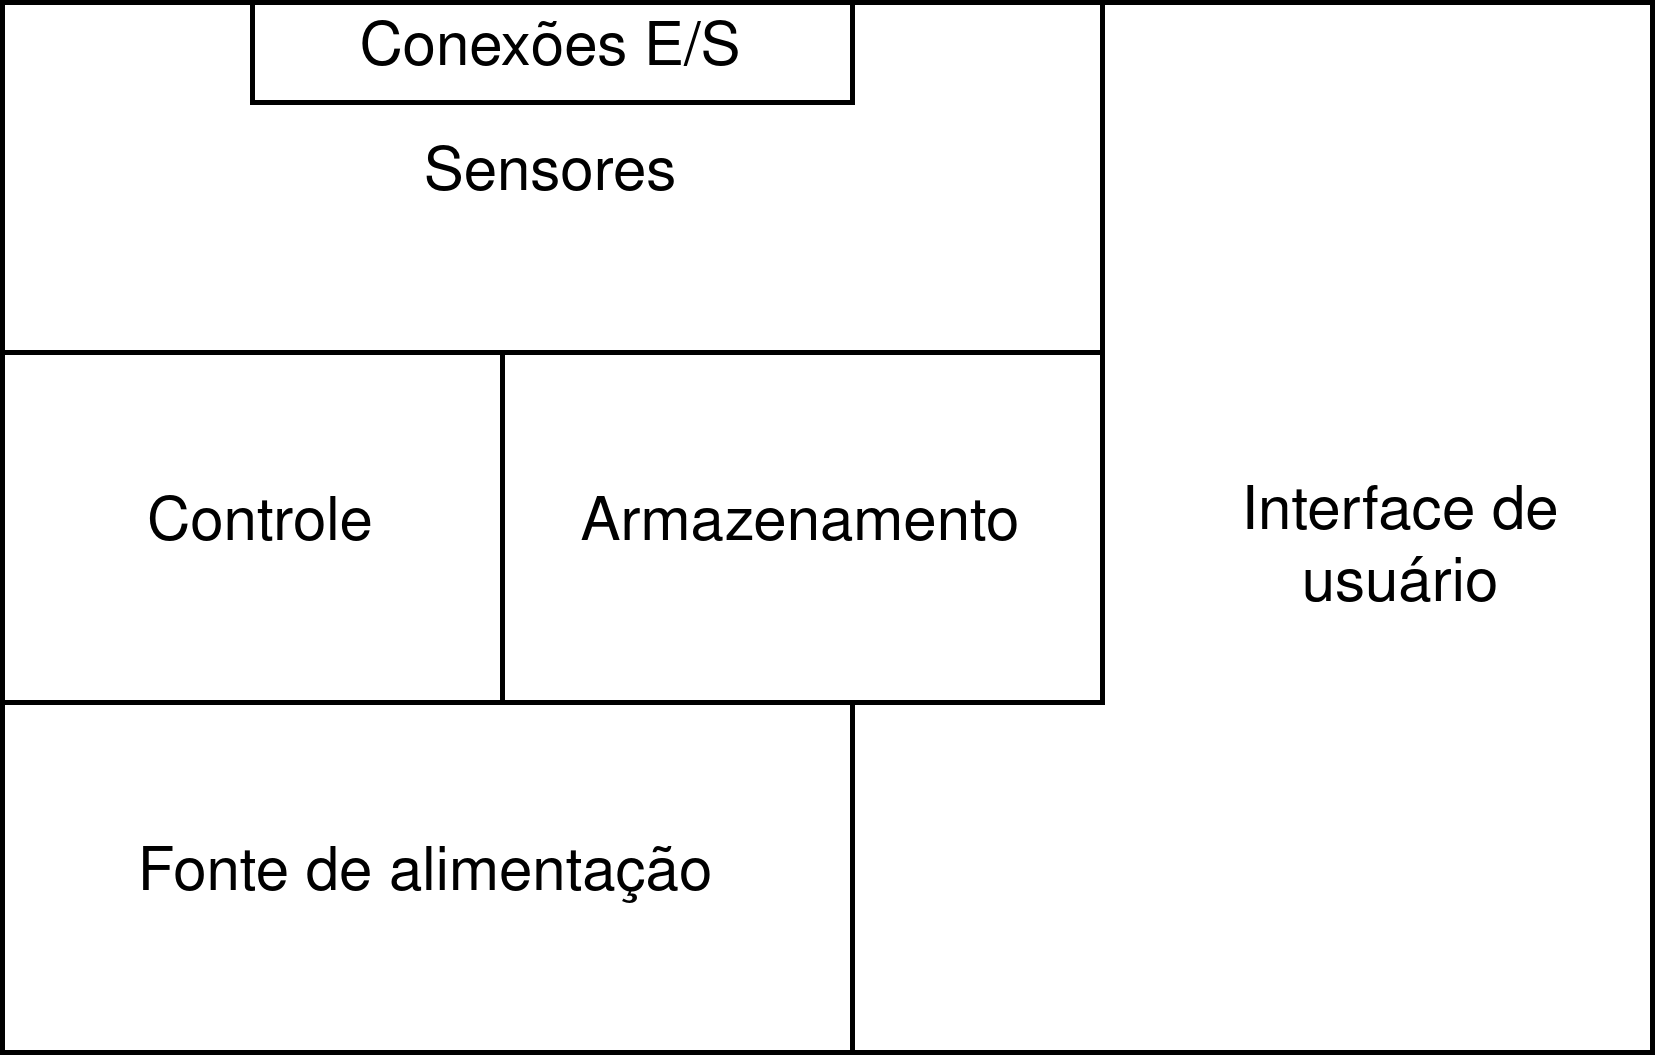
\includegraphics[width=\textwidth]{figuras/capitulo3/particionamento.drawio.png}}
    		}{
    			\Fonte{elaborado pelo autor (2022).}
    		}	
   \end{figure}


Em seguida fooram trazidos os desenhos dos componentes descritos nos esquemáticos eletrônicos para a visão de projeto PCB e dado início ao processo de organização dos componentes no espaço definido para a placa, com o circuito de controle sendo o primeiro a ser colocado e organizado nesse espaço.

Foi procurado posicionar o módulo microcontrolador no espaço que lhe foi reservado no particionamento, porém devido sua antena de comunicação Wi-Fi, foi seguida a recomendação da fabricante e o módulo foi posicionado de forma que a antena ficasse além das bordas da placa. Em seguida foram adicionados dois capacitores em paralelo com valores recomendados pela fabricante, paralelos a linha de alimentação do módulo para atuarem como um circuito de desacoplamento. Os demais componentes desse circuito que compõem o sub-circuito de habilitação de operação do módulo microcontrolador, foram posicionados também o mais próximo possível do módulo com exceção ao botão táctil e seus componentes auxiliares, que foram colocados na borda oposta da placa.

Em seguida, os componentes do circuito da fonte de alimentação do hardware foram colocados e posicionados de tal forma que O regulador de tensão U300 juntamente com seus componentes auxiliares foram posicionados próximos a linha de tensão do módulo microcontrolador a fim de atenuar interferências em sua alimentação. Os conectores desse circuito, juntamente com os componentes do sub-circuito foram posicionados próximos a borda da placa a fim de facilitar a conexão dos cabos de alimentação, mas também próximos o suficiente do regulador de tensão para evitar interferências em sua linha de alimentação. 

Os circuitos dos sensores foram colocados também na área que lhes foi reservada, com os sensores estando o mais próximo possíveis do módulo microcontrolador. Contudo, para os circuitos da interface de usuário e do leitor de cartão microSD não foi possível ajustar seus componentes de forma que fosse colocados exatamente nos espaços reservados no particionamento devido a sobreposição de algumas ligações desses circuitos.

Assim, o leitor de cartão microSD foi posicionado ao centro da placa de forma que ficasse oposto ao posicionamento do módulo microcontrolador. Para que fosse facilitado seu roteamento, o leitor foi colocado na face inferior da placa. Já os componentes do circuito de interface de usuário foram colocados o mais próximo das pontas das placa possível, de forma que também ficassem na mesma face mas do lado oposto ao módulo microcontrolador.


\subsubsection{Roteamento}

O processo de roteamento foi realizado utilizando-se inicialmente regras genéricas para tamanho de trilhas. Dessa forma, as trilhas inicialmente foram configuradas para possuírem 10 mil de largura. As primeiras trilhas a serem roteadas foram as conexões de comunicação e leitura de sensores devido sua importância em relação às demais conexões, assim pode-se ter maior liberdade de espaço para realizar o roteamento. 

Em seguida, realizou-se o roteamento do circuito de alimentação com o processo sendo iniciado pelas conexões dos sub-circuitos de entrada de alimentação e de seleção da fonte de alimentação. Tendo sido feitas as conexões de todos os componentes desse circuito, foi então dado início ao processo de conectar os demais circuitos da placa à alimentação.

Procurou-se fazer que houvesse uma trilha de alimentação que alcançasse maioria dos componentes realizando um contorno no sentido anti-horário ao redor do centro da placa. Foi escolhido essa estratégia em detrimento da criação de múltiplas trilhas de alimentação saindo de um ponto comum, para evitar a criação de vários pequenos ciclos de corrente ao longo da placa, o que poderia gerar interferências eletromagnéticas não só entre os circuitos do hardware mas também com o ambiente externo. 

Por fim foi realizado o roteamento dos componentes do circuito da interface de usuário, que foram tomados por último para esse processo devido suas conexões possuírem uma baixa complexidade. 



% \section{Definição da arquitetura de software}



% \subsection{Diagrama de blocos do software}


% \subsubsection{Diagrama organizacional de software}





\iffalse
-------------------------------------------------------------------------------------------------

% Texto texto texto texto texto texto texto texto texto texto texto texto texto texto texto texto texto texto texto texto texto texto texto texto texto texto texto texto texto texto texto texto texto texto texto texto texto texto texto texto texto texto texto texto texto texto texto texto texto texto texto texto texto texto texto texto texto texto texto texto texto texto texto texto texto texto texto texto texto.

% Texto texto texto texto texto texto texto texto texto texto texto texto texto texto texto texto texto texto texto texto texto texto texto texto texto texto texto texto texto texto texto texto texto texto texto texto texto texto texto texto texto texto texto texto texto texto texto texto texto texto texto texto texto texto texto texto texto texto texto texto texto texto texto texto texto texto texto texto texto.

\section{Exemplo de alíneas}\label{sec:exemplo-de-algoritmos-e-figuras}

    Texto texto texto texto texto texto texto texto texto texto texto texto texto texto texto texto texto texto texto texto texto texto texto texto texto texto texto texto texto texto texto texto texto texto texto texto texto texto texto texto texto texto texto texto texto texto texto texto texto texto texto texto texto texto texto texto texto texto texto texto texto texto texto texto texto texto texto texto texto.

    %\begin{algorithm}[h!]
    %	\SetSpacedAlgorithm
    %	\caption{\label{exemplo-de-algoritmo}Como escrever algoritmos no \LaTeX2e}
    %	\Entrada{o proprio texto}
    %	\Saida{como escrever algoritmos com  Latex:}% \LaTeX2e }
    %	\Inicio{
    %		inicialização;
    %		\Repita{fim do texto}{
    %			leia o atual;
    %			\Se{entendeu}{
    %				vá para o proximo\;
    %				próximo se torna o atual;}
    %			\Senao{volte ao início da seção;}
    %		}
    %	}	
    %\end{algorithm}

    Texto texto texto texto texto texto texto texto texto texto texto.

    %\begin{algorithm}[H]
    %	\Entrada{o proprio texto}
    %	\Saida{como escrever algoritmos com \LaTeX2e }
    %	\Inicio{
    %		inicialização\;
    %		\Repita{fim do texto}{
    %			leia o atual\;
    %			\Se{entendeu}{
    %				vá para o próximo\;
    %				próximo se torna o atual\;}
    %			\Senao{volte ao início da seção\;}
    %		}
    %	}
    %	\caption{Exemplo de Algoritmo Versao 02}
    %\end{algorithm}

    %\begin{algorithm}
    %	\begin{algorithmic}
    %	\Entrada{o proprio texto}
    %	\Saida{como escrever algoritmos com \LaTeX2e }	
    %	\end{algorithmic}
    %\end{algorithm}

    Exemplo de alíneas com números:

    \begin{alineascomnumero}
	    \item Texto texto texto texto texto texto texto texto texto texto texto texto .
	    \item Texto texto texto texto texto texto texto texto texto texto texto texto .
	    \item Texto texto texto texto texto texto texto texto texto texto texto texto .
	    \item Texto texto texto texto texto texto texto texto texto texto texto texto .
	    \item Texto texto texto texto texto texto texto texto texto texto texto texto .
	    \item Texto texto texto texto texto texto texto texto texto texto texto texto .
    \end{alineascomnumero}

    Texto texto texto texto texto texto texto texto texto texto texto texto texto texto texto texto texto texto texto texto texto texto texto texto texto texto texto texto texto texto texto texto texto texto texto texto texto texto texto texto texto texto texto texto texto texto texto texto texto texto texto texto texto texto texto texto texto texto texto texto texto texto texto texto texto texto texto texto texto.

    Ou então figuras podem ser incorporadas de arquivos externos, como é o caso da \autoref{fig-grafico-1}. Se a figura que ser incluída se tratar de um diagrama, um gráfico ou uma ilustração que você mesmo produza, priorize o uso de imagens vetoriais no formato PDF. Com isso, o tamanho do arquivo final do trabalho será menor, e as imagens terão uma apresentação melhor, principalmente quando impressas, uma vez que imagens vetorias são perfeitamente escaláveis para qualquer dimensão. Nesse caso, se for utilizar o Microsoft Excel para produzir gráficos, ou o Microsoft Word para produzir ilustrações, exporte-os como PDF e os incorpore ao documento conforme o exemplo abaixo. No entanto, para manter a coerência no uso de software livre (já que você está usando LaTeX e abnTeX),  teste a ferramenta InkScape\index{InkScape}. ao CorelDraw\index{CorelDraw} ou ao Adobe Illustrator\index{Adobe! Illustrator}.  De todo modo, caso não seja possível  utilizar arquivos de imagens como PDF, utilize qualquer outro formato, como JPEG, GIF, BMP, etc.  Nesse caso, você pode tentar aprimorar as imagens incorporadas com o software livre \index{Gimp}Gimp. Ele é uma alternativa livre ao Adobe Photoshop\index{Adobe! Photoshop}.

\section{Usando Fórmulas Matemáticas}

Para escrever um símbolo matemático no texto, escreva símbolo entre cifrões, por exemplo, $\alpha$, $\beta$ e $\gamma$ são símbolo do alfabeto grego. Se você quiser inserir equações enumeradas, siga a estrutura de
\begin{equation}
    \label{eq:indices}
	k_{n+1} = n^2 + k_n^2 - k_{n-1}.
\end{equation}
Observe a pontuação, pois a equação faz parte da frase e do parágrafo. Como a equação faz parte da frase, não se utiliza o \textit{label} numérico \ref{eq:indices}. 

Quando for citar a Equação \ref{eq:indices} novamente no texto, utiliza-se o \textit{label} numérico. Repare que a palavra ``Equação'' foi escrita com ``E'' maiúsculo. 

Um exemplo de equações com frações é dado por
\begin{equation}
	\label{eq:fracao}
		\begin{aligned}
			x = a_0 + \cfrac{1}{a_1
				+ \cfrac{1}{a_2
					+ \cfrac{1}{a_3 + \cfrac{1}{a_4} } } }.
		\end{aligned}
	\end{equation}

Texto texto texto texto texto texto texto texto texto texto texto texto texto texto texto texto texto texto texto texto texto texto texto texto texto texto texto texto texto texto texto texto texto texto texto texto texto texto texto texto texto texto texto texto texto texto texto texto texto texto texto texto texto texto texto texto texto texto texto texto texto texto texto texto texto texto texto texto texto
	\begin{equation}
		\begin{aligned}
			k_{n+1} = n^2 + k_n^2 - k_{n-1}.
		\end{aligned}
	\end{equation}
	
Texto texto texto texto texto texto texto texto texto texto texto texto texto texto texto texto texto texto texto texto texto texto texto texto texto texto texto texto texto texto texto texto texto texto texto texto texto texto texto texto texto texto texto texto texto texto texto texto texto texto texto texto texto texto texto texto texto texto texto texto texto texto texto texto texto texto texto texto texto
	\begin{equation}
	\label{eq:trigo}
		\begin{aligned}
			\cos (2\theta) = \cos^2 \theta - \sin^2 \theta
		\end{aligned}.
	\end{equation}
	
Texto texto texto texto texto texto texto texto texto texto texto texto texto texto texto texto texto texto texto texto texto texto texto texto texto texto texto texto texto texto texto texto texto texto texto texto texto texto texto texto texto texto texto texto texto texto texto texto texto texto texto texto texto texto texto texto texto texto texto texto texto texto texto texto texto texto texto texto texto
	\begin{equation}
	\label{eq:matriz}
		\begin{aligned}
			A_{m,n} =
			\begin{pmatrix}
			a_{1,1} & a_{1,2} & \cdots & a_{1,n} \\
			a_{2,1} & a_{2,2} & \cdots & a_{2,n} \\
			\vdots  & \vdots  & \ddots & \vdots  \\
			a_{m,1} & a_{m,2} & \cdots & a_{m,n}
			\end{pmatrix}
		\end{aligned}.
	\end{equation}

Texto texto texto texto texto texto texto texto texto texto texto texto texto texto texto texto texto texto texto texto texto texto texto texto texto texto texto texto texto texto texto texto texto texto texto texto texto texto texto texto texto texto texto texto texto texto texto texto texto texto texto texto texto texto texto texto texto texto texto texto texto texto texto texto texto texto texto texto texto
	\begin{equation}
	\label{eq:sistema}
		\begin{aligned}
			f(n) = \left\{ 
			\begin{array}{l l}
			n/2 & \quad \text{if $n$ is even}\\
			-(n+1)/2 & \quad \text{if $n$ is odd}
			\end{array} \right.
		\end{aligned}.
	\end{equation}
Texto texto texto texto texto texto texto texto texto texto texto texto texto texto texto texto texto texto texto texto texto texto texto texto texto texto texto texto texto texto texto texto texto texto texto texto texto texto texto texto texto texto texto texto texto texto texto texto texto texto texto texto texto texto texto texto texto texto texto texto texto texto texto texto texto texto texto texto texto

%\section{Usando Algoritmos}

%\begin{algorithm}[h!]
%	\SetSpacedAlgorithm
%	\caption{\label{alg:algoritmo_de_colonica_de_formigas}Algoritmo de Otimização por Colônia de Formiga}
%	\Entrada{Entrada do Algoritmo}
%	\Saida{Saida do Algoritmo}
%	\Inicio{
%		Atribua os valores dos parâmetros\;
%		Inicialize as trilhas de feromônios\;
%		\Enqto{não atingir o critério de parada}{
%			\Para{cada formiga}{
%				Construa as Soluções\;
%			}
%			Aplique Busca Local (Opcional)\;
%			Atualize o Feromônio\;
%		}	
%	}		
%\end{algorithm}

\section{Usando Código-fonte}

Um exemplo de código-fonte, ou código de programação encontra-se no Apendice \ref{ap:A}

 
\section{Usando Teoremas, Proposições, etc}

 Texto texto texto texto texto texto texto texto texto texto texto texto texto texto texto texto texto texto texto texto texto texto texto texto texto.

\begin{teo}[Pitágoras]
	Em todo triângulo retângulo o quadrado do comprimento da
	hipotenusa é igual a soma dos quadrados dos comprimentos dos catetos. Usando o Apêndice \ref{ap:C}
\end{teo}


Texto texto texto texto texto texto texto texto texto texto texto texto texto texto texto.

\begin{teo}[Fermat]
	Não existem inteiros $n > 2$, e $x, y, z$ tais que $x^n + y^n = z$
\end{teo}

Texto texto texto texto texto texto texto texto texto texto texto texto texto texto texto.

\begin{prop}
	Para demonstrar o Teorema de Pitágoras...
\end{prop}

Texto texto texto texto texto texto texto texto texto texto texto texto texto texto texto.

\begin{exem}
	Este é um exemplo do uso do ambiente exem definido acima.
\end{exem}

Texto texto texto texto texto texto texto texto texto texto texto texto texto texto texto.


\begin{xdefinicao}
	Definimos o produto de ...
\end{xdefinicao}

Texto texto texto texto texto texto texto texto texto texto texto texto texto texto texto.

\section{Usando Questões} 

Um exemplo de questionário encontra-se no Apêndice \ref{ap:B}.

%Movido para o Apêndice

\fi